% Figure 1 vector source (standalone; compile with -jobname=fig1_calibergraph).
% 177.2mm wide. All in-figure text >= 9pt Helvetica; global line width 0.5pt.
% Color semantics: green=witnessed/answer, red=gap/refuse, blue=compiled modules &
% contract-bound slots, orange=typed graph & compile, gray=external/candidate-origin.
% Grayscale redundancy: shapes, line styles, check/cross, hatch. The linker is the only
% online-LLM component; determinism is carried by panel (d)'s "0 online calls" statement.
\documentclass[10pt]{standalone}
\usepackage{helvet}
\usepackage{tikz}
\usetikzlibrary{arrows.meta,positioning,fit,patterns}
\usepackage{amssymb}
\usepackage{pifont}
\begin{document}
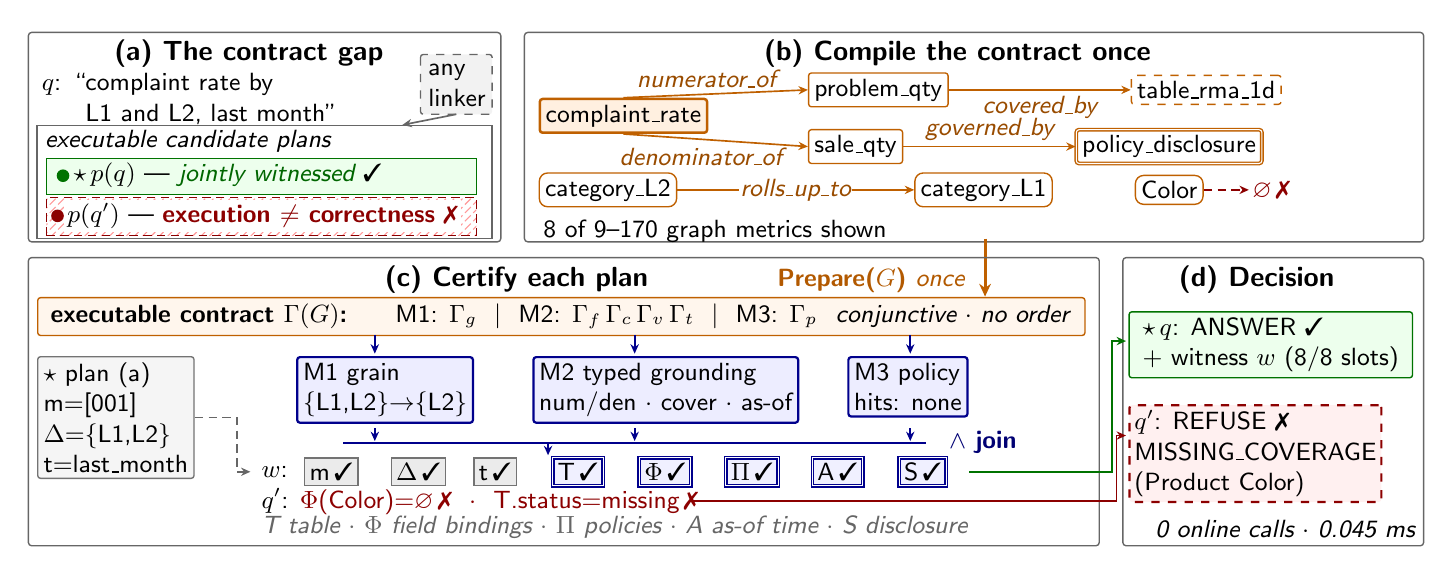
\begin{tikzpicture}[x=1mm,y=1mm, line width=0.5pt,
  every node/.style={font=\small\sffamily, inner sep=1.5pt, align=left},
  ptitle/.style={font=\normalsize\bfseries\sffamily, inner sep=0pt, anchor=north},
  panel/.style={draw=black!60, rounded corners=1.2pt},
  box/.style={draw, rounded corners=1pt, inner sep=2.1pt},
  gnode/.style={box, draw=orange!75!black, font=\small\sffamily},
  extbox/.style={box, dashed, draw=black!60, fill=black!5},
  modbox/.style={box, thick, draw=blue!55!black, fill=blue!7, anchor=north west},
  cchip/.style={draw=black!55, inner sep=1.8pt, fill=black!8},
  kchip/.style={draw=blue!55!black, inner sep=1.8pt, double, double distance=0.4pt, fill=blue!6},
  gapzone/.style={draw=red!55!black, densely dashed, pattern=north east lines, pattern color=red!40},
  okzone/.style={draw=green!45!black, fill=green!7},
  arr/.style={-{Stealth[length=3.4pt,width=3pt]}, semithick},
  oarr/.style={arr, orange!75!black},
  barr/.style={-{Stealth[length=4.6pt,width=4.2pt]}, line width=1.1pt, orange!75!black},
  elbl/.style={font=\small\itshape\sffamily, inner sep=0.5pt, fill=white, text=orange!60!black},
  note/.style={font=\small\itshape\sffamily}]

% ============ canvas ============
\path (0,-4.2) rectangle (177.2,-70.6);

% ================= (a) THE CONTRACT GAP =================
\draw[panel] (0,-4.8) rectangle (60,-31.4);
\node[ptitle] at (28,-5.7) {(a) The contract gap};
\node[anchor=north west] at (1.1,-9.4) {$q$: ``complaint rate by\\\hphantom{$q$: ``}L1 and L2, last month''};
\draw[dashed, black!60, fill=black!5, rounded corners=1pt] (49.8,-7.6) rectangle (58.9,-15.2);
\node[anchor=north east, inner sep=2.1pt] at (58.9,-8.1) {any\\linker};
% zone diagram: stacked witnessed / gap bands
\draw[black!60] (1.1,-16.6) rectangle (58.9,-31.0);
\node[anchor=north west, note] at (1.5,-16.65) {executable candidate plans};
\node[okzone, anchor=north west, minimum width=54.6mm, minimum height=4.6mm] at (2.2,-20.7) {};
\fill[green!45!black] (4.4,-23.0) circle (0.8);
\node[anchor=west, inner sep=1pt] at (5.3,-23.0) {$\star\,p(q)$ --- {\itshape\color{green!40!black}jointly witnessed}~\ding{51}};
\node[gapzone, anchor=north west, minimum width=54.6mm, minimum height=4.8mm] at (2.2,-25.7) {};
\fill[red!55!black] (3.7,-28.1) circle (0.8);
\node[anchor=west, inner sep=1pt, fill=white] at (4.5,-28.1) {$p(q')$ --- {\bfseries\color{red!55!black}execution $\neq$ correctness}~{\color{red!55!black}\ding{55}}};
\draw[arr, black!60] (54.35,-15.2) -- (47.5,-16.55);

% ================= (b) COMPILE ONCE =================
\draw[panel] (63,-4.8) rectangle (177.2,-31.4);
\node[ptitle] at (118,-5.7) {(b) Compile the contract once};
% typed graph (staggered rows)
\node[gnode, line width=0.9pt, fill=orange!12, anchor=west] (gm) at (64.8,-15.4) {complaint\_rate};
\node[gnode, anchor=west] (gnum) at (99,-12.1) {problem\_qty};
\node[gnode, anchor=west] (gden) at (99,-19.3) {sale\_qty};
\node[gnode, dashed, anchor=west] (gtb) at (140,-12.1) {table\_rma\_1d};
\node[gnode, double, double distance=0.4pt, anchor=west] (gpo) at (133,-19.3) {policy\_disclosure};
\node[gnode, rounded corners=3pt, anchor=west] (gl2) at (64.8,-24.8) {category\_L2};
\node[gnode, rounded corners=3pt, anchor=west] (gl1) at (112.5,-24.8) {category\_L1};
\node[gnode, rounded corners=3pt, anchor=west] (gcol) at (140.5,-24.8) {Color};
\node[anchor=west, inner sep=1pt, text=red!55!black] (gnull) at (155,-24.8) {$\varnothing$\,\ding{55}};
\draw[oarr] (gm.north) -- (gnum.west) node[elbl, pos=0.45, above=1.6pt] {numerator\_of};
\draw[oarr] (gm.south) -- (gden.west) node[elbl, pos=0.42, below=2.4pt] {denominator\_of};
\draw[oarr] (gnum.east) -- (gtb.west) node[elbl, midway, below=1.6pt] {covered\_by};
\draw[oarr] (gden.east) -- (gpo.west) node[elbl, midway, above=1.4pt] {governed\_by};
\draw[oarr] (gl2.east) -- (gl1.west) node[elbl, midway] {rolls\_up\_to};
\draw[oarr, densely dashed, red!55!black] (gcol.east) -- (gnull.west);
\node[note, anchor=north west, font=\small\sffamily] at (64.8,-28.0) {8 of 9--170 graph metrics shown};
% Prepare(G) once: exits (b), enters the Gamma bus of (c)
\draw[barr] (121.5,-31.0) -- (121.5,-38.35);

% ================= (c) CERTIFY EACH PLAN =================
\draw[panel] (0,-33.4) rectangle (136,-70.0);
\node[ptitle] at (62,-34.3) {(c) Certify each plan};
\node[anchor=east, font=\small\bfseries\sffamily, text=orange!70!black] at (119.5,-36.3) {Prepare($G$) {\mdseries\itshape once}};
% Gamma bus
\node[box, draw=orange!75!black, fill=orange!7, anchor=north west, minimum width=133mm, minimum height=4.8mm] (gbus) at (1.1,-38.4) {};
\node[anchor=west, font=\small\bfseries\sffamily] at (2.2,-40.8) {executable contract $\Gamma(G)$:};
\node[anchor=west] at (46,-40.8) {M1: $\Gamma_g$ ~$\vert$~ M2: $\Gamma_f\,\Gamma_c\,\Gamma_v\,\Gamma_t$ ~$\vert$~ M3: $\Gamma_p$};
\node[anchor=east, note] at (132.8,-40.8) {conjunctive $\cdot$ no order};
% star candidate card (4 lines, narrow left column)
\node[box, draw=black!55, fill=black!4, anchor=north west] (card) at (1.1,-45.9) {$\star$ plan (a)\\m=[001]\\$\Delta$=\{L1,L2\}\\t=last\_month};
% three parallel modules
\node[modbox] (m1) at (34,-45.9) {M1 grain\\\{L1,L2\}$\to$\{L2\}};
\node[modbox] (m2) at (64,-45.9) {M2 typed grounding\\num/den $\cdot$ cover $\cdot$ as-of};
\node[modbox] (m3) at (104,-45.9) {M3 policy\\hits: none};
\draw[arr, blue!55!black] (44,-43.2) -- (44,-45.6);
\draw[arr, blue!55!black] (77,-43.2) -- (77,-45.6);
\draw[arr, blue!55!black] (112,-43.2) -- (112,-45.6);
% join bar (M3 drops vertically like M1/M2; bar extended under M3)
\draw[line width=0.8pt, blue!55!black] (40,-56.9) -- (114,-56.9);
\draw[arr, blue!55!black] (44,-55.1) -- (44,-56.7);
\draw[arr, blue!55!black] (77,-55.1) -- (77,-56.7);
\draw[arr, blue!55!black] (112,-55.1) -- (112,-56.7);
\node[anchor=west, font=\small\bfseries\sffamily, inner sep=1pt, text=blue!45!black] at (116.5,-56.9) {$\wedge$ join};
\draw[arr, blue!55!black] (66,-57.1) -- (66,-58.5);
% plan card feeds the candidate-origin slots of the witness row
\draw[arr, black!60, densely dashed] (card.east) -| (26.5,-60.6) -- (28.2,-60.6);
% witness board
\node[anchor=west] at (29,-60.6) {$w$:};
\node[cchip, anchor=west] at (35,-60.6) {m\,\ding{51}};
\node[cchip, anchor=west] at (46,-60.6) {$\Delta$\,\ding{51}};
\node[cchip, anchor=west] at (56.5,-60.6) {t\,\ding{51}};
\node[kchip, anchor=west] at (66.5,-60.6) {T\,\ding{51}};
\node[kchip, anchor=west] at (77.5,-60.6) {$\Phi$\,\ding{51}};
\node[kchip, anchor=west] at (88.5,-60.6) {$\Pi$\,\ding{51}};
\node[kchip, anchor=west] at (99.5,-60.6) {A\,\ding{51}};
\node[kchip, anchor=west] at (110.5,-60.6) {S\,\ding{51}};
\node[anchor=west] at (29,-64.35) {$q'$: {\color{red!55!black}$\Phi$(Color)=$\varnothing$\,\ding{55} ~$\cdot$~ T.status=missing\,\ding{55}}};
% slot gloss row (P1-6): meanings match the Task-section witness definition
\node[anchor=west, note, text=black!60] at (29,-67.7) {T table $\cdot$ $\Phi$ field bindings $\cdot$ $\Pi$ policies $\cdot$ A as-of time $\cdot$ S disclosure};

% ================= (d) DECISION =================
\draw[panel] (139,-33.4) rectangle (177.2,-70.0);
\node[ptitle] at (156,-34.3) {(d) Decision};
\node[box, draw=green!45!black, fill=green!7, anchor=north west, minimum width=36mm] (ans) at (139.7,-40.2) {$\star\,q$: ANSWER \ding{51}\\+ witness $w$ (8/8 slots)};
\node[box, draw=red!55!black, thick, dashed, fill=red!6, anchor=north west, inner sep=1.8pt] (ref) at (139.7,-52.0) {$q'$: REFUSE \ding{55}\\MISSING\_COVERAGE\\(Product Color)};
\draw[arr, green!45!black] (119.5,-60.6) -| (137.6,-44.0) -- (139.4,-44.0);
\node[note, anchor=south east] at (176.7,-69.6) {0 online calls $\cdot$ 0.045 ms};
\draw[arr, red!55!black] (84,-64.35) -- (138.2,-64.35) (138.2,-64.35) |- (139.4,-56.0);
\end{tikzpicture}
\end{document}
